\documentclass{article}
\usepackage{tikz}

\begin{document}

\begin{center}
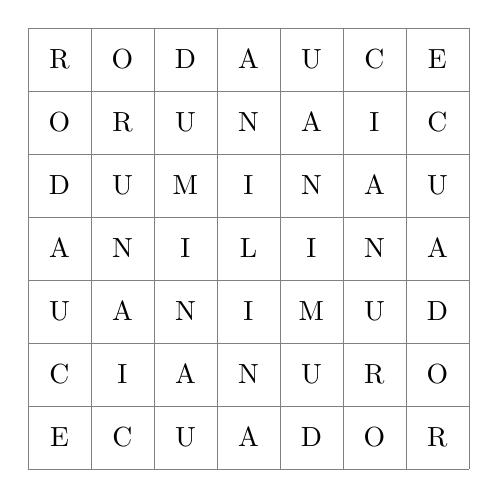
\begin{tikzpicture}[scale=0.8]
    \draw[help lines] (0,0) grid (7,7);
    
    \foreach \row [count=\y from 0] in {
        {E,C,U,A,D,O,R},
        {C,I,A,N,U,R,O},
        {U,A,N,I,M,U,D},
        {A,N,I,L,I,N,A},
        {D,U,M,I,N,A,U},
        {O,R,U,N,A,I,C},
        {R,O,D,A,U,C,E}}
    {
        \foreach \col [count=\x from 0] in \row
        {
            \node at (\x+0.5,\y+0.5) {\col};
        }
    }
\end{tikzpicture}
\end{center}

\textbf{Description:} Satorian Square of dimension \( n = 7 \). It is built with three Spanish words: ECUADOR, CIANURO (cyanide), and ANILINA (aniline), and one word that has no meaning: UANIMUD.

\end{document}